\section{From first certification to a traded fund}
\label{sec:full-strategy}
The fixed-reference experiment cannot establish fund performance after entry.
We therefore freeze a separate full-strategy study, preserving every earlier
result. It uses the same financial DGP, estimation windows, turnover/impact
parameters, leverage and annual Forward--Backward--Swap10 priority. Its six
methods are All Signals, Greedy, repeated HAC, constant-bound Catoni, geometric
corrected-tail betting and the one-period Oracle. All four selection methods
start empty; each actual fund pays its own costs and its performance includes
all time spent waiting in cash. The Oracle's weights are constructed from
current moments before drawing the return shock. It receives no future shock
or coefficient path.

The tail method retains the nine scale/fraction pairs already declared. Its
geometric moment bounds now use the difference and sum of general candidate
and reference stock exposures, with their exact predictable cost difference.
No true coefficient, regime or conditional gain enters the bets. The common
episode-mean floor is $10^{-8}$ daily utility, ranking ties within $10^{-9}$
use stable signal identifiers, and the QP tolerance is $10^{-10}$. Empty and
single-coordinate allocations are computed exactly. These declared numerical
conventions distinguish this study from the earlier positive-only baseline;
all four new selection methods share them. The pilot pool, 50001--50100, was
declared before the initial implementation's markets. A numerical failure in
its final block for seed 50005 led us to retain the initial outputs as
diagnostics and replay the same pool with corrected arithmetic: allocation
differences are formed before projections, and $Y$ is evaluated as
$d(1-\gamma s/2)-D$. This preserves the exact economic score and all design
parameters; it avoids erasing a tiny contrast next to a large common position.
The failed seed is included in the replay and no seed is counted twice.
This is a pilot software correction, not an additional independent experiment.
Final seeds 60001--60500 remain separate and unobserved at protocol freeze.
The subsequent expanded v2 pilot stopped at seed 50020 when its QP failed
the required convergence status despite refinement. Nineteen markets had
completed. The table below remains the prespecified first-ten snapshot;
the failed market is retained and the full pilot is not claimed complete.
A further numerical revision expresses the same QP objective in basis points
after failed refinement and checks its original-unit KKT conditions. It
completes the failed market; the entire pilot is being replayed with unchanged
economic parameters. The fund table here retains the first-ten v2 snapshot
and does not combine implementation versions as extra replications.
In all nineteen complete markets shared by v2 and v3, the audited fund/score
ledgers, event labels, decisions and metrics match byte for byte. The first
three sealed blocks of the previously failed market match as well. Every
configuration field agrees apart from its version label. This cross-version
equality check is distinct from independent arithmetic replay and supplies
no additional market replications.

\subsection{Economic events that retain early responses}
An economic opportunity starts at the end of the first annual block with
positive evaluator conditional mean utility difference. It qualifies as stable
only if the unchanged support pair, following its own allocation states and
the common expanding-fit rule, has a positive mean in the following block.
Inception-positive opportunities and subsequent sign changes are distinct.
The delay has annual resolution: zero means selection at that first annual
review, not instantaneous recognition of an unobserved daily change.

If selection, a competing move or shortlist withdrawal closes a comparison
before its second block, evaluator-only copies of both shadow policies
continue for that block. One additional evaluator year resolves pending
onsets at the main horizon. The continuation's allocations, utilities and
true-mean labels are evaluator outputs and never feed the learner or its
betting capital. Ordinary market returns within the main horizon still update
the common estimation history; the extra year is excluded from that history
and from actual fund returns. Separate optimizer
instances prevent evaluator queries from changing learner warm starts.
This construction includes fast responses in the same stability denominator
as slower responses. Confirmed events terminate at selection, a competing
move, shortlist withdrawal, economic sign reversal or the administrative
horizon; those causes are retained separately.

Meeting a statistical criterion differs from winning the annual ranking.
We therefore report criterion detection and actual selection separately, with
ENTRY, PARK, REVIVE and SWAP lifecycle labels. Within-one/three/five-year
fractions require the corresponding full calendar follow-up for every onset,
including successful onsets. Competing closures are not treated as independent
administrative censoring. These are descriptive, method-specific opportunity
populations; they are neither common causal risk sets across methods nor
labels for T1's conditional null. Sparse or absent PARK/REVIVE events cannot
support a claim of successful regime adaptation.

A separate deployment ledger evaluates the next selected action from the
actual previous fund allocation. It compares the new and retained-support
weights from the same state under next-period true moments, before drawing
that period's shock. This evaluator quantity diagnoses deployment quality;
the historical test does not certify it. Its horizon is one day: a negative
initial gain can coexist with a positive subsequent holding value after the
entry cost is amortized. It is not a classification of lifetime trade value;
the full fund utility paths address performance over the study horizon.
A choice made at the final review
is logged as terminal and contributes no executed trade or subsequent fund
performance.

\subsection{Numerical verification and executed evidence}
The evaluator computes general score moments by writing
$d=(w_B-w_S)'A$ and $s=(w_B+w_S)'A$, so
$Y=d-\gamma ds/2-D$. For independent standardized Laplace shocks, the joint
cumulant of orders $(a,b)$ of their centered parts is zero when $a+b$ is odd
and, for even $a+b=2k\ge2$, equals
\[
 \kappa_{a,b}=\frac{(2k)!}{k2^k}
       \sum_l h_{d,l}^{a}h_{s,l}^{b}.
\]
The usual moment--cumulant recurrence then gives all terms needed for
$\E Y^2$ and $\E Y^4$. Difference exposures are formed before computing
moments to avoid subtracting nearly identical large fourth-order terms.
Independent polynomial convolution and conditional Monte Carlo check this
calculation. Actual code checks the public geometric certificates against
these evaluator-only moments; they are not used to choose the certificate.

An independent arithmetic replay loads saved compact policy weights and
recreates the market without loading checkpoints or test-process states.
It reconstructs fund wealth, utility and costs; candidate/reference scores
and costs; predictable certificates and bets; nine-component tail capitals;
annual eligibility and priority selections; and counterfactual event means.
This verifies numerical consistency, while proof validity, economic utility
and global error control remain separate questions.

\IfFileExists{generated_full_results.tex}{The reported full-strategy pilot snapshot contains 100 completed independent markets (0 requested snapshot markets remain incomplete). Each has 500 stocks, 100 signals, one training block and 14 out-of-sample blocks of 252 days. Independent arithmetic replay covers 100 of these completed markets. These are pilot observations; the separate 500-market final study is not asserted to be complete. Earlier baseline and fixed-reference markets, and later markets outside the specified snapshot, are not added to this count.

\begin{table}[H]\centering\small

\begin{tabular}{lrrrr}

\toprule

Method & $h\bar U$ (MC SE) & Mean wealth & Inactive & Mean moves \\

\midrule

All Signals & 0.04429 (0.00113) & 1.889 & 0.000 & 0.00 \\

Greedy & 0.05166 (0.00074) & 2.083 & 0.071 & 6.47 \\

HAC & 0.05100 (0.00075) & 2.064 & 0.071 & 2.87 \\

Catoni & 0.00000 (0.00000) & 1.000 & 1.000 & 0.00 \\

Tail & 0.01104 (0.00043) & 1.170 & 0.821 & 0.99 \\

Oracle & 0.05844 (0.00050) & 2.282 & 0.000 & 0.00 \\

\bottomrule\end{tabular}

\caption{Full-strategy pilot means. Utility is daily utility rescaled by $h=252$, not an annual certainty equivalent. MC SE uses independent markets. Wealth includes waiting in cash and all modeled actual fund costs. Moves include terminal choices, which create no post-choice fund return.}\end{table}

Tail makes 99 choices (ENTRY: 99, PARK: 0, REVIVE: 0, SWAP: 0), of which 99 are executed before the horizon. Its mean inactive fraction is 0.821. Successful initial certification therefore must be assessed alongside the returns foregone during waiting. The lifecycle counts delimit what this pilot can say about parking and revival.

\begin{table}[H]\centering\small

\begin{tabular}{lrrr}

\toprule

Method & Eligible stable events & Criterion within year & Selected within year \\

\midrule

Greedy & 7515 & 6435 & 368 \\

HAC & 5962 & 3788 & 199 \\

Catoni & 4787 & 0 & 0 \\

Tail & 4760 & 0 & 0 \\

\bottomrule\end{tabular}

\caption{Response-independent stable-event cohorts with a full year of calendar follow-up. Each row has its own endogenous reference policies and event population; raw counts do not identify causal cross-method detection performance. Dependent events are not treated as independent replications.}\end{table}

\begin{table}[H]\centering\small

\begin{tabular}{lrrrr}

\toprule

Method & Executed & Positive gain & Mean gain (bp) & Entry cost (bp) \\

\midrule

Greedy & 620 & 0.140 & -0.712 & 1.190 \\

HAC & 285 & 0.305 & -0.256 & 1.291 \\

Tail & 99 & 1.000 & 0.931 & 1.500 \\

\bottomrule\end{tabular}

\caption{Evaluator-only next-period gains from the actual previous allocation, including modeled transition costs. These descriptive outcomes concern executed decisions, exclude terminal certifications, and are not quantities certified by a historical episode rejection.}\end{table}

\begin{figure}[H]\centering

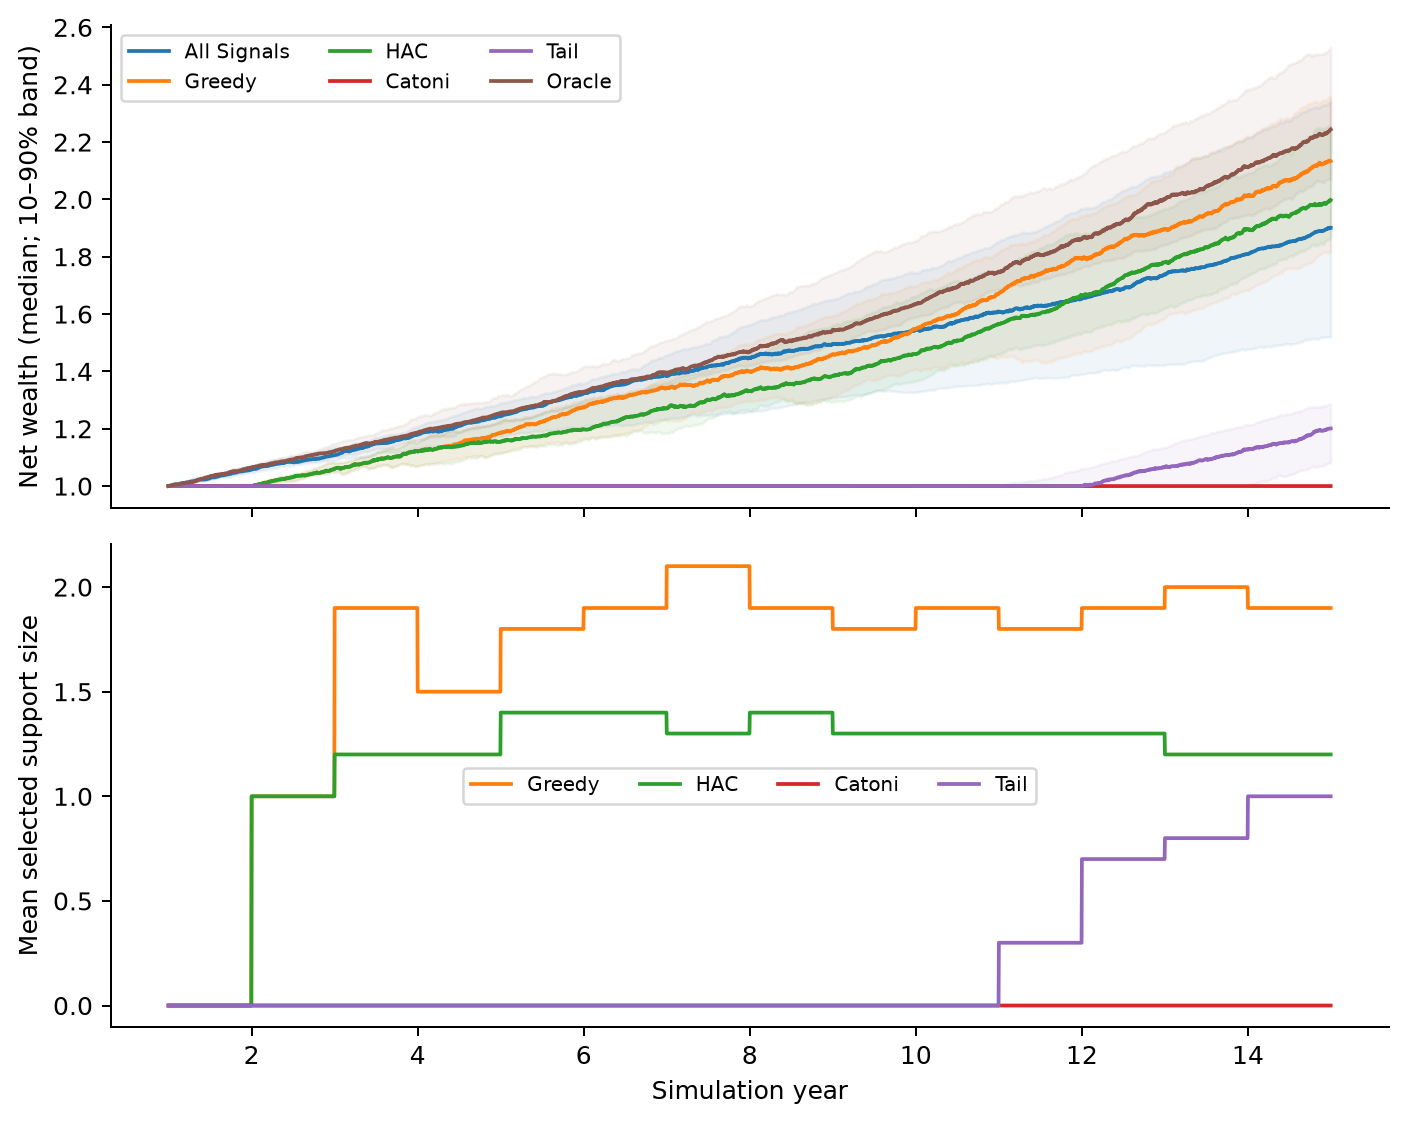
\includegraphics[width=.96\linewidth]{figures/full_strategy_paths.png}

\caption{Actual net wealth and selected support size in the completed full-strategy pilot. Wealth bands are the 10th and 90th market percentiles; they are descriptive quantiles, not confidence intervals.}

\end{figure}

\begin{figure}[H]\centering

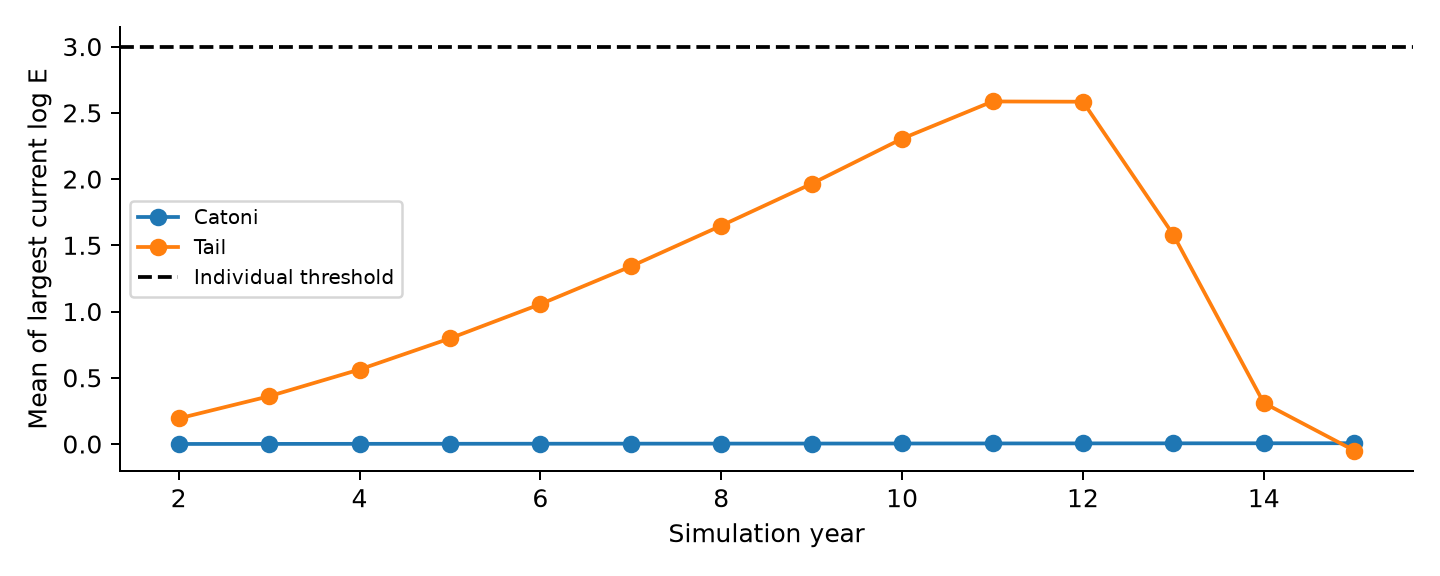
\includegraphics[width=.96\linewidth]{figures/full_strategy_evidence.png}

\caption{Mean across completed markets of the largest currently open annual log capital. Closed comparisons are not carried forward. The dashed line is the individual threshold; it does not protect the entire search.}

\end{figure}

Paired Tail-minus-reference differences in $h\bar U$ (95\% Student MC intervals) are All Signals: -0.03325 [-0.03560, -0.03089]; Greedy: -0.04062 [-0.04187, -0.03938]. These exploratory intervals use independent paired markets and are unadjusted across comparisons; they do not give guarantees for a new financial law. The reproducibility tables retain every benchmark contrast.

All Signals permits every candidate but does not hold all of them: its mean number of positions exceeding $10^{-6}$ in absolute sleeve weight is 4.54. This descriptive count is computed after the run and changes no allocation or test. The optimizer already produces a sparse portfolio, so it is a substantive baseline for the value of an additional statistical support filter. No fixed per-signal research cost is charged in this design.

Catoni executes a move in 0 of 100 markets (Wilson 95\% interval for the market-level fraction [0.000, 0.037]). A zero observed fraction does not establish zero probability of future entry.
}{
No completed full-strategy result is asserted by this version of the draft.}
\FloatBarrier
